\chapter{Teoretická část}
%Some introductory text\dots

\section{Stávající metody}
\subsection{Předzpracování}
\subsubsection{Binární obraz}
Většina metod se zakládá na zpracování binárního obrazu. Probíhá to zvolením prahové hodnoty, se kterou se všechny hodnoty porovnají a ve výsledku vznikne binární obraz. Objekt, který je středem zájmu, se skládá z pixelů s hodnotou 1 zatímco ostatní mají hodnotu 0.
\subsubsection{Rozostření}
Rozostření slouží jako relativně spolehlivá eliminace šumu v obraze. Nejosvědčenější metody jsou pomocí Gausse nebo mediánu.\\

Filtr medián se zaměřuje na vyhlazování lokálních extrémů z obrazu. Nejprve se seřadí všechny hodnoty z aktuální konvoluční matice a vybere hodnotu, která leží uprostřed seřazeného pole a tou nahradí zpracovávaný bod. Velikost okolí zahrnutého v analýze se může zvětšit při větší hustotě šumu~\cite{15}. Ale v aplikaci na hloubkový obraz, ve kterém se detekují prsty je důležité zachovat určité rozlišení.\\
\begin{figure}[h]
\centering
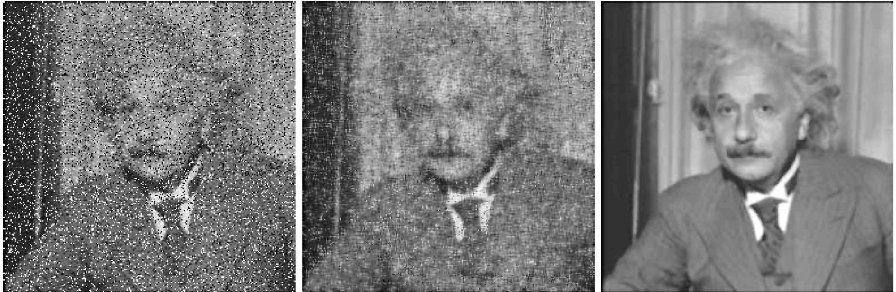
\includegraphics[width=0.8\linewidth]{median.jpg}
\caption{a) původní obraz b) průměrování c) medián
Rozdíl mezi filtrem s průměrováním a mediánem 
~\cite{15} }
\end{figure}


Gaussův filtr je průměrování s Gaussovským rozložením~\cite{15}. Využívá se k vyhlazování obrazu a odstranění detailů a šumu. 
\begin{eqnarray}
G(x,y) = \frac{1}{2 \pi \sigma^{2}}*e^{-\frac{x^{2}+y^{2}}{2\sigma^{2}}}
%ae^{-\frac{(x-b)^{2}}{2c^{2}}}
\end{eqnarray}

Proti rozšíření do nekonečna se v konvoluční masce přidělí větší váha bodu ve středu. Aby se aplikací konvoluční masky neměnila světlost, součet všech složek konvoluční matice dává hodnotu 1. Příklad konvoluční masky:
\begin{eqnarray}
\frac{1}{16} \begin{bmatrix}
1 & 2 & 1 \\
2 & 4 & 2 \\
1 & 2 & 1
\end{bmatrix}
\end{eqnarray} 

\begin{figure}[h]
\centering
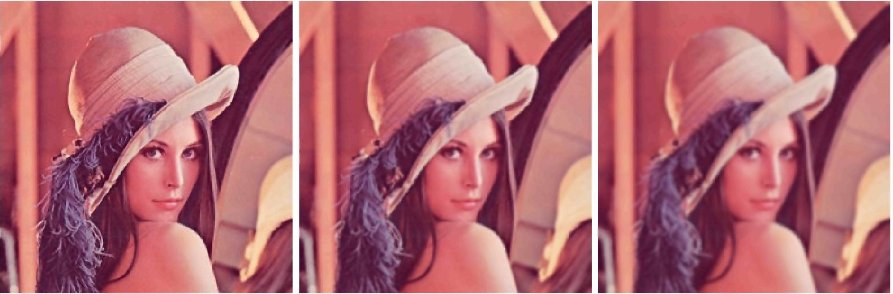
\includegraphics[width=0.8\linewidth]{gauss.jpg}
\caption{a) původní obraz b) jednou aplikovaný Gaussův filtr c) třikrát aplikovaný Gaussův filtr~\cite{15} }
\end{figure}




\subsection{Rozpoznávání postav}
Možnosti:

podle tvaru
\begin{itemize}
\item na základě modelu
\item na základě prvků

\item strojově naučené programy
\item neuronové sítě %-radial basis funkction
\item transformační matice vzdálenostních funkcí (chamfer)
\end{itemize}

podle barvy
\begin{itemize}
\item strojově naučené programy\\
\end{itemize}


Jednou z metod je dle Ch. Nakajima a spol.~\cite{6} ukládání několika obrázků, z nichž se detekuje pohybující se objekt a vše, co se nehýbe se označí za pozadí a ignoruje. Následně se naleznou kraje možné postavy, aby se vylepšil výsledek a vymazal šum. Pokud se jedinec pohybuje v druhém kroce, oříznutí probíhá z posledního získaného obrazu. Pokud nebyl detekován žádný jedinec, tak se do paměti uloží pozadí, které se z následujících obrazů rovnou vymaže pro větší přesnost. K vlastní identifikaci se použila SVM (support vector machines) a k-NN klasifikátor.\\

Hussein a spol.~\cite{9}používají k rozpoznání postavy prohledávání obrazu a porovnávání siluet s databází, ve které jsou vzory lidských postav. Shoda je detekována pomocí zkosením objektů. Vzory jsou ve formě binárního obrazu. Vzdálenost D mezi vzorem V a objektem z obrazu O se počítá vzorcem\\

\begin{eqnarray}
 D(O,V) = \frac{1}{|V|}\sum_{i}^{}C_{i}V_{i} ,
\end{eqnarray}

kde |V| je počet pixelů v siluetě ve vzoru, $ T_{i} $ je hodnota pixelu $ i $ ve vzoru a $ C_{i} $ je rozdíl zkosení pixelu $ i $ v obraze. Čím menší hodnota mezi vzorem a obrazem, tím lepší shoda je detekována.
%// (patří do nového odstavce?)

Nalezení podobnosti zkosením předpokoládá již nalezené hrany objektů v obraze. Vzor se překryje co nejvíce na objekt a transformací bodů jednoho objektu pomocí parametrických tramsformačních rovnic.\\

Jiný přístup poskytuje nalezení objektu v zorném poli pomocí hloubkové kamery, následným rozhodnutím, zda objekt má lidské nohy, nebo aspoň dva objekty odpovídající tvaru, a pokud ano, tak se přejde k dalšímu kroku, ve kterém se detekuje barva kůže z RGB vstupu. Nalezený výsledek slouží jako oblast k detekci obličeje, čímž je definitivně nalezen člověk~\cite{10}.\\

Gavrila ~\cite{7} se snaží snížit výpočetní náročnost tak, že nahrazuje procházení obrazu postupně schopností zaměřit se na jeden úryvek přímo a ve druhém kroce teprve hledá podobnosti tvarů. Dosahuje tak zpracování v reálném čase.
%These pixel values form a distribution of distances of the template features to the nearest features in the image
Shodu podle tvaru detekuje pomocí vzdálenosti křivek, která se počítá podobně jako u Hussein a spol.~\cite{9} 

\begin{eqnarray}
 D(O,V) = \frac{1}{|V|}\sum_{t\in T}^{}d_{I}(t) ,
\end{eqnarray}
kde |V| je počet prvků ve vzoru a $ d_{I}(t) $ představuje vzdálenost daného prvku ve vzoru a odpovídajícímu v obraze. Pokud výslená hodnota je menší, než předem určená prahová hodnota, považuje se objekt v obraze za postavu. 
%hlubší pozornost na předposlední odstavec na str. 4 !!!!

\begin{figure}[h]
\centering
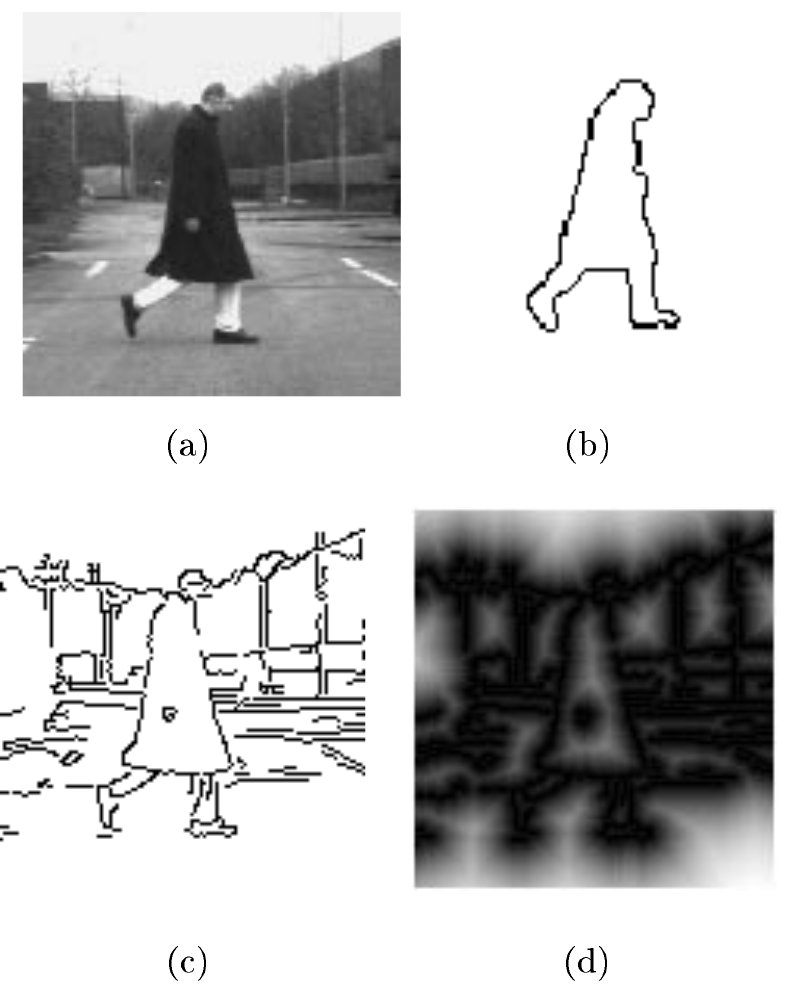
\includegraphics[width=0.6\linewidth]{pedestrian_detection.jpg}
\caption{a) původní obraz b) vzor c) nalezené hrany d) vyobrazené vzdálenosti~\cite{7} }
\end{figure}

V rámci optimalizace se tato metoda (jak překládat chemfer matching system??) rozšiřuje na hierarchizovanou, která sdružuje podobné vzory do shluků a tudíž se prohledávání databáze zrychlí.
\begin{figure}[h]
\centering
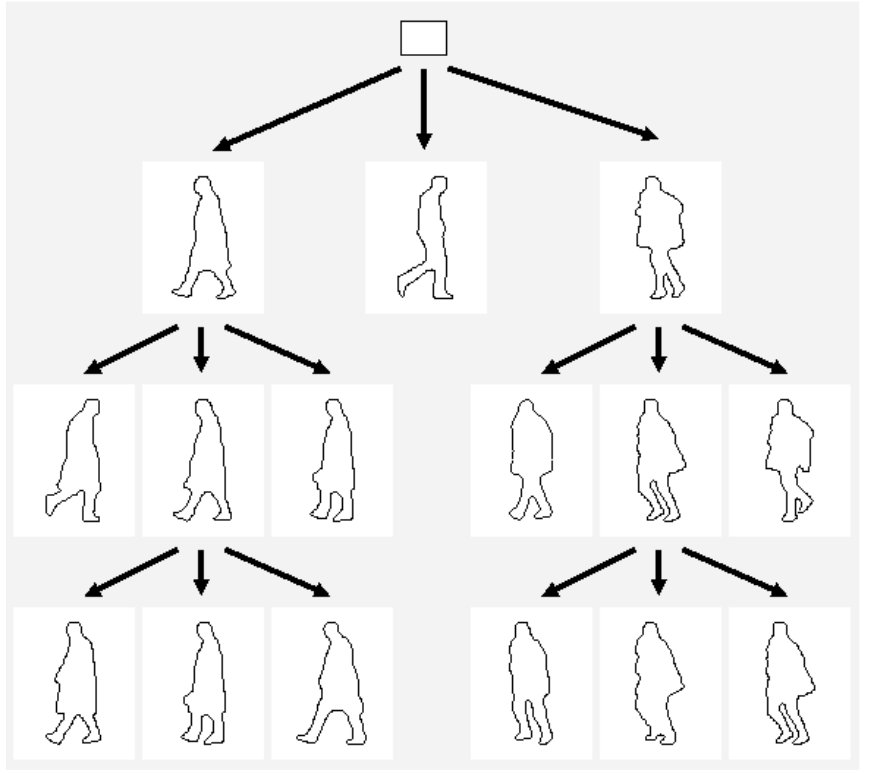
\includegraphics[width=0.6\linewidth]{hier.jpg}
\caption{využití hierarchie v databázi vzorů~\cite{7} }
\end{figure}

Ověření výsledku probíhá RBF (radial basis functions) klasifikátorem. Nejdříve se z původního obrazu vybere čtyřúhelník obsahující možnou postavu a na základě euklidovské vzdálenosti určuje, jestli jednotlivé pixely jsou součástí postavy či nikoliv.\\
%RBF classifier!

Riggol a spol.~\cite{11} kombinují rozpoznávací metody založené na prvcích a na modelech za cílem dosažení spolehlivého a efektivního programu. Využívají P2DHMM (Pseudo-2D Hidden Markov Model). Jedná se o předem naučený algoritmus, který dokáže na základě pravděpodobností určit, jestli se jedná o postavu nebo ne.\\
\begin{figure}[h]
\centering
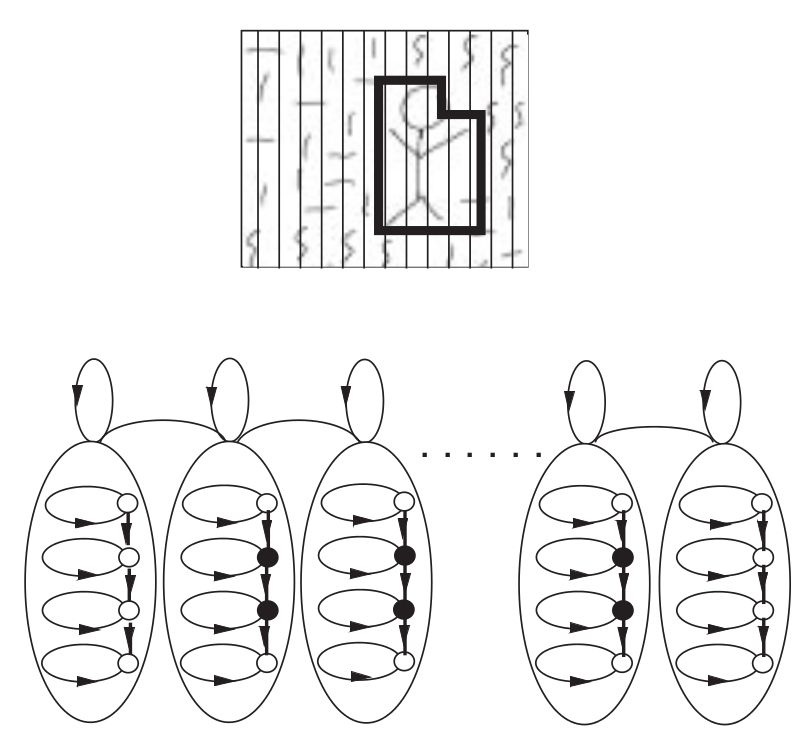
\includegraphics[width=0.5\linewidth]{P2DHMM.jpg}
\caption{stochastický model 2D objektu ~\cite{11} } %stochastic model of 2D object using P2DHMM
\end{figure}


\subsection{Rozpoznávání částí těla}
%Hledání rukou na základě~\cite{10} :\\
%	vzhledu (barva, tvar)\\ 
%	naučené(learning based) -kNN,..\\
%			-Haarovy cascades\\
Ruka má 23 stupňů vlastností a v kombinaci s různým osvětlením a změnami v pozadí se jedná o značně komplikovaný problém na řešení pomocí podobnosti.\\

Jestliže aplikace nevyžaduje dynamické využití, lze použít rozdíl mezi objektem a pozadím~\cite{14}. Vyžaduje to co nejvíce neměnné pozadí a dostatečný rozdíl mezi objektem a zbytkem. Rozdíl lze hledat jednoduše procházením pole nebo využitím "chytrého" algoritmu. Spočívá v identifikaci čísti obrazu, která se hýbe oproti posledním obrazům.
\begin{figure}[h]
\centering
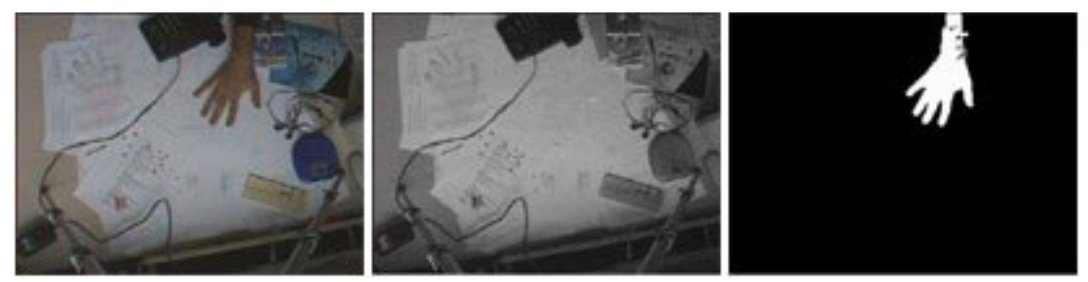
\includegraphics[width=1\linewidth]{diff.jpg}
\caption{a)vstup  b) referenční obraz  c)výstup ~\cite{14} } 
\end{figure}


\subsection{Rozpoznávání gest}
Mezi rozpoznávání na základě vzhledu se řadí mnoho metod zahrnujících strojově naučené algoritmy jako neuronové sítě, HMM (Skrytý Markovův model) a jiné~\cite{3}. Gesto lze identifikovat i pomocí extrakce (ČESKY) pozice a směru ruky a jednotlivých prstů.\\

Kim a spol.~\cite{5} používají bílé značky na špičkách prstů, které sledují černým světlem a detekují jednoznačně špičky prstů, což umožňuje velkou škálu možných gest. Na druhou stranu vzniká i omezení barvy pozadí, které lze eliminovat jen v uričtém prostředí, tudíž se jedná o vhodnou variantu k využití při hrách ve VR (virtuální reality).\\

Shaker a Zliekha ~\cite{12} získávají směr prstu na ruce, kterou snímají dvěmi kamerami. Jedna kamera natáčí shora, zatímco druhá zboku. Oba vstupy se zpracovávají zvlášť do rozpoznávání gesta. Nejdříve přepočítají obraz na stupně šedi a poté dle určené prahové hodnoty odfiltruje pozadí a vytvoří binární obraz. V tomto kroce je třeba, aby bylo pozadí jednoduché a jasně rozlišitelné od ruky. Kvůli odstanění šumu se obrázek rozmaže a následně zaostří. V tomto kroce vzniká podmínka, že největší objekt v obraze je právě ruka. Poté se pomocí Laplaciána získají hrany daného objektu a z něj se vytvoř kontury.
Gesto se identifikuje pomocí nalezení největšího vrcholu v obraze a nalezení čáry, kterou opisuje natažený prst a následnou kombinací obou směrů do 3D. 
\begin{figure}[h]
\centering
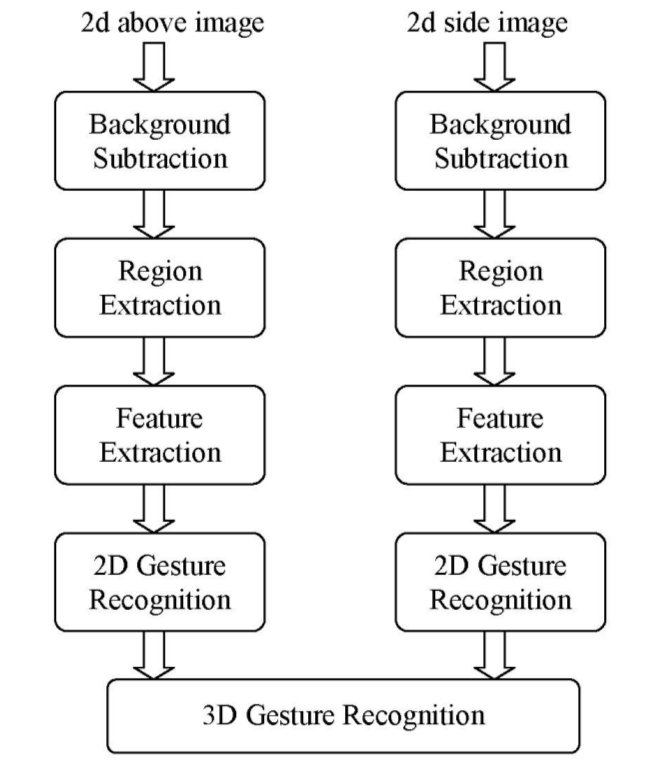
\includegraphics[width=0.5\linewidth]{ShZl.jpg}
\caption{popis algoritmu~\cite{12} } 
\end{figure}

\subsubsection{Rozpoznávání prstů}
Hackenberg a spol.~\cite{12} implementovali identifikaci prstů a dlaně na základě několika kroků. Nejprve projde hloubkový obraz z kamery a hledá tvary podobné špičkám prstů nebo rourovitého tvaru podobného prstům. Poté se zaměří na detailnější vlastnosti dlaně. Z nalezených vhodných polí, která mohou představovat dlaňě se vyřadí ta, která nejsou napojena nijak na prsty, jsou menší než předem určená hodnota (odvozená od průměrně velikosti hlavy) a vzdáleností špiček prstů od dlaně.\\


Bez potřeby porovnávání tvarů a zdrojů se dají rozpoznat jednotlivé špičky prstů pomocí nalezení lokálního maxima v obrysu ruky. Ve všech adekvátních směrech se naleznou kandidáti a následně vyloučí mylné identifikace. Jedná se ale o postup náchylný k šumu v obraze, podobná metoda odolnější navrhuje porovnávání vzdálenosti obrysu k pozici ruky~\cite{3}.\\
Jednotlivé prsty lze rozpoznat například pomocí vyhledávání na základě tvaru~\cite{4}. Jde o zjednodušení představy objektu na geometrický objekt a vyhledávání vhodných kandidátů v obraze. 
%obrázek figertip jako geometrického objektu ze zdroje?

Mezi další programy rozpoznávající špičky prstů z již relativně čistého čtyřúhelníku, který obsahuje zájmový objekt, patří identifikace na základě dvou specifickách vlastností. Centrum špičky je obklopen kolem pixelů patřící prstu a ten je obklopen dlouhou řadou pixelů nepatřících prstu~\cite{14}. Ruce lze identifikovat i až po prstech a to tak, že se vyloučí objekty podobného tvaru (propisky, fixy), které nesplňují vlastnosti rukou, například nepatří k žádné dlani.




\begin{figure}[h]
\centering
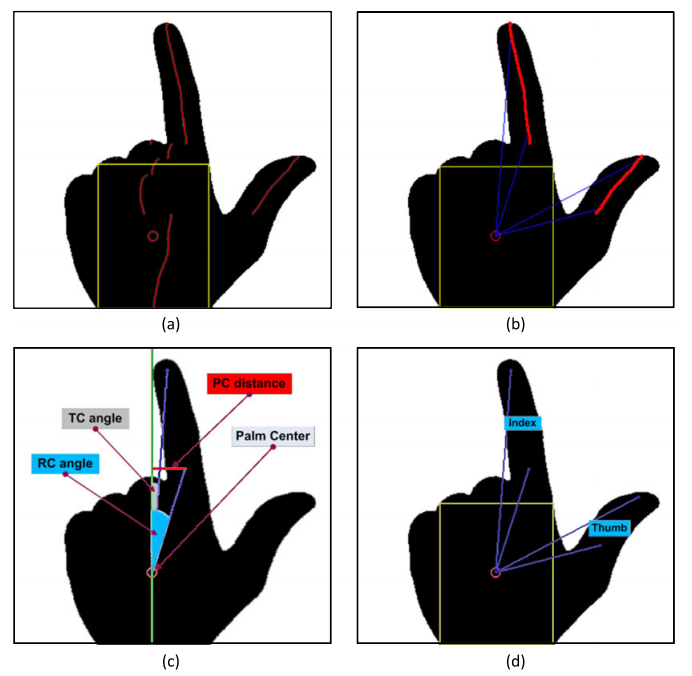
\includegraphics[width=0.5\linewidth]{fingers.png}
\caption{Vyobrazení definovaných pojmů, které lze využít k výpočtům pozic, na základě proporcionálních vlastností prstů. ~\cite{13} }

\end{figure}
\begin{center}
$RC_{angle} = 90 - tan^{-1} \frac{y_{r}-y_{pc}}{x_{r} - x_{pc}}$ \\
$TC_{angle} = 90 - tan^{-1} \frac{y_{ft}-y_{pc}}{x_{ft} - x_{pc}}$ 
\end{center}
\section{Aktuální aplikace}
Všechny aplikace, které mohou využít výhod~\cite{14}:
\begin{itemize}
\item Ovládání na velmi malém prostoru
\item Ovládání z větší vzdálenosti
\item Snížený počet součástek
\item Zjednodušené ovládání elektroniky
\item Potenciál zabezpečení proti zneužití (při implementaci ochranných prvků)
\item Minimalistické (méně tlačítek a obdobných prvků)\\
\end{itemize}
Potenciál pro využití v:
\begin{itemize}
\item Překlad znakové řeči
\item Ovládání chytrých zařízení (chytrá domácnost - světla, hudba, televize, telefon)
\item Prezentace před publikem (ovládání počítače)
\\
\end{itemize}
Již využíváno v:
\begin{itemize}
\item Rozpoznání chodce v dohledu vozidla
\item Sociální experimenty (vyslání robota stopovat)
\item Ovládání a hraní na konzolích
\end{itemize}



\endinput
%%
%% End of file `ch01.tex'.
